\documentclass[10pt, twocolumn]{article}

\input{template.tex}

\title{Towards a random-based approach for synthetic pandas query generation}

\author{
  Liam Scalzulli \\
  McGill University \\
  \href{mailto:liam.scalzulli@mail.mcgill.ca}{liam.scalzulli@mail.mcgill.ca}
}

\date{\today}

\begin{document}

\maketitle

\begin{abstract}
  This paper presents a random-based procedural algorithm for synthetic pandas query generation. We show that this approach, although vastly simple, can be used to generate valid and complex queries, suitable for processes in data science
  and machine learning, such as evaluating database systems,
  predicting cardinality, and estimating execution times.
\end{abstract}

\section{Introduction}

\textbf{pandas} is a data analysis library for Python that provides a fast and efficient DataFrame object for data manipulation with integrated indexing.

\spacing
\noindent
A DataFrame is two-dimensional, size-mutable, potentially heterogeneous tabular data. We can easily create them from native Python structures:

\begin{verbatim}
>>> d = {'col1': [1, 2], 'col2': [3, 4]}
>>> df = pd.DataFrame(data=d)
>>> df
   col1  col2
0     1     3
1     2     4
\end{verbatim}

\noindent
We can write queries against this dataframe (df) using familiar Python syntax.

\spacing
\noindent
Selection ($\sigma$) filters rows based on boolean conditions:

\begin{verbatim}
>>> df[df['col1'] > 1]
   col1  col2
1     2     4
\end{verbatim}

\noindent
Projection ($\pi$) selects specific columns:

\begin{verbatim}
>>> df[['col1']]  # Select only col1
   col1
0     1
1     2
\end{verbatim}

\noindent
Merging ($\bowtie$) combines DataFrames based on common columns:

\begin{verbatim}
>>> df1 = pd.DataFrame({'key': ['A'], 'val1': [1]})
>>> df2 = pd.DataFrame({'key': ['A'], 'val2': [3]})
>>> df1.merge(df2, on='key')
  key  val1  val2
0   A     1     3
\end{verbatim}

\noindent
GroupBy ($\gamma$) operations aggregate data by specified columns:

\begin{verbatim}
>>> df = pd.DataFrame({
...   'group': ['A', 'A', 'B', 'B'],
...   'value': [1, 2, 3, 4]
... })
>>> df.groupby(by=['group']).agg('sum')
       value
group
A          3
B          7
\end{verbatim}

\noindent
These fundamental operations form the basis for more complex queries that can be generated by our algorithm. When combined, they enable sophisticated data manipulation and analysis capabilities.

\section{Problem Statement}
The generation of synthetic database queries presents several
key challenges that this work aims to address:

\begin{enumerate}
  \item \textbf{Query Validity}: Generated queries must be
    syntactically correct and logically consistent, ensuring
    they can execute successfully against real datasets.

  \item \textbf{Human-like Structure}: The queries should
    reflect patterns commonly used by data analysts, avoiding
    artificial or unrealistic constructions that might bias
    downstream applications.

  \item \textbf{Complexity Control}: The generation process
    should support varying levels of query complexity, from
    simple operations to multi-stage transformations combining
    multiple DataFrame operations.
\end{enumerate}

\noindent
Formally, given a DataFrame schema $S$, parameters that constrain the query generation process $P_{Q}$, and a set of valid
pandas operations $O = \{\sigma, \pi, \bowtie, \gamma\}$, we
aim to generate a query $Q$ such that:

\begin{itemize}
  \item $Q$ is a valid composition of operations from $O$, satisfying the constraints given by $P_{Q}$.
  \item $Q$ produces a non-empty result set when executed on data conforming to schema $S$.
  \item $Q$ exhibits structural similarities to human-written queries in terms of operation frequency and complexity.
\end{itemize}

\noindent
Our solution focuses on a randomized approach that balances
simplicity with effectiveness, while maintaining control over
the statistical properties of the generated queries.

\section{Algorithm}

The algorithm is concerned with solving the query generation problem in the most simple manner. To achieve this we leverage a wide array of user input to guide our generation steps, using random number generators where applicable.

\subsection*{Input}

To start, we accept a schema $S$. This schema gives us meta-data about the data we're generating queries for. It contains information such as the primary keys for tables, foreign key relationships, column information, etc. This information guides us throughout the various sub-algorithms employed for each operation type.

\spacing
\noindent
Moreover, we accept a few parameters that describe the structure of individually generated queries:

\begin{itemize}
  \item Maximum number of selection conditions ($C_{\sigma}$).
  \item Probability of generating a selection ($P_{\sigma}$).
  \item Maximum number of projection columns ($C_{\pi}$).
  \item Probability of generating a projection ($P_{\pi}$).
  \item Maximum number of merge operations ($N_{\bowtie}$).
  \item Maximum number of group-by columns ($C_{\gamma}$).
  \item Maximum number of aggregation columns ($C_{\Sigma}$).
  \item Probability of generating a group-by ($P_{\gamma}$).
\end{itemize}

\noindent
These components inform us what to do during the core query building step of the algorithm.

\subsection*{State}

We maintain a few state variables throughout the algorithm:

\begin{itemize}
  \item Entity ($E$). The acting entity of the query being generated.
  \item The currently available columns ($C$).
  \item The required columns ($R$). Used when orchestrating projection operations.
  \item Merge entities ($M$). A set of entities that this query is composed of.
\end{itemize}

\noindent
By definition, $R \subseteq C$ holds throughout the life-cycle of the algorithm.

\subsection*{Query Building}

The query building step in the algorithm decides which operation we should be generating, based on the input parameters described above.

\spacing
\noindent
The pseudo-code for this procedure is described as follows:

\spacing
\begin{lstlisting}
if |C| > 0 and $C_{\sigma}$ > 0 and rand() < $P_{\sigma}$
  generate a selection

if |C| > 0 and $C_{\pi}$ > 0 and rand() < $P_{\pi}$
  generate a projection

from 0 to rand(0, $N_{\bowtie}$)
  if we can generate a merge, do it
  otherwise give up

if |C| > 0 and $C_{\gamma}$ > 0 and rand() < $P_{\gamma}$
  generate a group by operation
\end{lstlisting}

\spacing
\noindent
This procedure constrains the generated query in a few subtle ways:

\begin{itemize}
  \item Each individually generated query can have \textbf{at most} 1 selection and 1 projection operation. Generated queries can have sub-queries, so the total amount will vary.
  \item A group by operation is always generated at the end, allowing us to tweak query parameters to ensure we only append one at the end of the outer-most query. This will become more apparent once we describe the merge generation process.
\end{itemize}

\noindent
These subtle constraints are in place because we want generated queries to exhibit structural similarities to human-written queries. Without these constraints, we could generate queries with all sorts of bizarre operation patterns, such as a multitude of projections one after the other.

\subsection*{Operation Types}

As seen above, the query building step dispatches to our individual operation generation algorithms. In this section, we describe the algorithm for each operation type. Our working set of operations is assumed to be $\{\sigma, \pi, \bowtie, \gamma\}$.

\subsubsection*{Selection $(\sigma)$}

Selections, alongside merges, are one of the trickier operations to generate.

\spacing
\noindent
A purely random approach to generating conditions could yield nonsensical results, culminating in an empty intersection. For instance, if we're generating conditions for an entity with an integer property $x$, a possible condition set could be $x < 5 \land x > 10$.

\spacing
\noindent
The goal is to generate a condition set that satisfies the constraints imposed by $C_{\sigma}$ and is logically consistent (no empty intersections).

\spacing
\noindent
Assume the data types and the data ranges for each column on all tables are given by schema $S$. We can proceed with a base algorithm:

\spacing
\begin{lstlisting}
set $COND$ to be an empty list

set $X$ to be rand(1, min($C_{\sigma}$, |C|))

from 1 to $X$
  pick a random column $C_{i}$ $\in$ $C$

  set $T_{i}$ to the type of column $C_{i}$
  set $R_{i}$ to be the range of column $C_{i}$

  generate and append a condition that considers $T_{i}$, $R_{i}$ and references $C_{i}$, to $COND$

select on the condition set $COND$
\end{lstlisting}

\spacing
\noindent
Next we describe generating conditions and adding them to $COND$, while maintaining consistency of the entire condition set.

\spacing
\noindent
Consistency conflicts can only be generated when operating on the same value. For instance, a possible solution to this problem would be to cap the number of conditions per column to 1. Since we want to avoid doing this, we have to figure out a way to satisfy the desired number of conditions while maintaining consistency.

\spacing
\noindent
We approach this problem by keeping track of previously generated conditions for columns, and grouping conditions for each column in parentheses, joined by random operations. For example, a valid condition set would look like (x $\textgreater$ 3 $\land$ x $\textless$ 10) $\lor$ (y = 5) $\land$ (z $\geq$ 10 $\lor$ z $\leq$ 40).

\spacing
\noindent
(TODO: Finish this section with a described algorithm)

\subsubsection*{Projection $(\pi)$}

A projection operation simply selects out of our available columns set $C$ a random subset to project. Before we do this however, we subtract the required column set $R$ from the available columns, appending them right before generating the projection:

\spacing
\begin{lstlisting}
set $P$ to $C$ - $R$

if $P$ is empty
  project $C$

set $X$ to rand(1, min($C_{\pi}$ - |R|, len($P$)))

select a subset $P_{S} \subseteq P$, $|P_{S}| = X$

set $C$ to $P_{S}$ + $R$

project $P_{S}$ + $R$
\end{lstlisting}

\subsubsection*{Merge $(\bowtie)$}

Merge operations are special in the sense that they can produce sub-queries. For instance, inspect the following query:

\begin{verbatim}
nation.merge(
  region[(region['R_NAME'] != 'M')],
  left_on='N_REGIONKEY',
  right_on='R_REGIONKEY'
)
\end{verbatim}

\noindent
We merge the entity $nation$ with rows in $region$ whose $R\_NAME$ property is not equal to $M$.

\spacing
\noindent
Assume we can get foreign key relationships from $S$ by an entity $E$ ($S[E]$). These are given as tuples ($c_{l}$, $c_{f}$, $\varepsilon$) where $c_{l}$ is the local column on $E$, $c_{f}$ is the foreign column and $\varepsilon$ is the foreign entity (or table) containing $c_{f}$.

\spacing
\noindent
We use all of this information to suggest a recursive approach, which is outlined in the following algorithm:

\spacing
\begin{lstlisting}
set $E_{C}$ to an empty list

for $c_{l}$, $c_{f}$, $\varepsilon$ from $S[E]$
  if $c_{l} \in C$
    add $c_{l}$, $c_{f}$, $\varepsilon$ to $E_{C}$

if $E_{C}$ is empty
  give up, we can't perform a merge

choose a $c_{l}$, $c_{f}$, $\varepsilon$ $\in E_{C}$

set X to be a new empty query on $\varepsilon$

set parameters for $X$
  $P_{\gamma}$ = 0 // Ensures we have no groupby
  $N_{\bowtie}$ = $N_{\bowtie}$ - # merges for this query
  ... inherit from the current query

build a query $X$ with $R$ + $\{c_{f}\}$, $C$ = all columns on $\varepsilon$

set $C$ to the union of $C$ with the columns returned by $X$

set $M$ to the union of $M$ with the merge entities of query $X$

subtract $N_{\bowtie}$ by the number of merges in query $X$

merge the current query with $X$
\end{lstlisting}

\spacing
\noindent
To get a feel for how this algorithm works, lets take a look at the relational algebra tree for the example query shown above:

\spacing
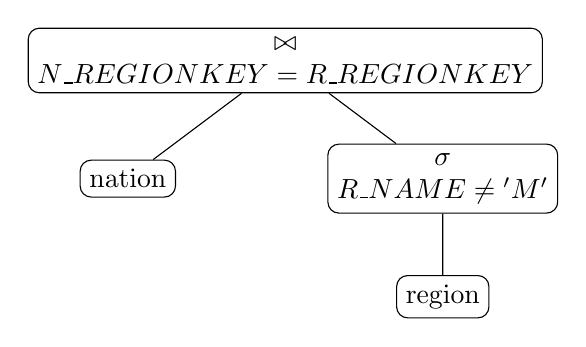
\begin{tikzpicture}[
  level distance=1.5cm,
  level 1/.style={sibling distance=4cm},
  level 2/.style={sibling distance=3cm},
  every node/.style={draw, rounded corners, align=center}
]
\node{$\bowtie$\\$N\_REGIONKEY = R\_REGIONKEY$}
  child {
    node {nation}
  }
  child {
    node {$\sigma$\\$R\_NAME \neq \text{'M'}$}
      child {
        node {region}
      }
  };
\end{tikzpicture}

\spacing
\noindent
Our algorithm starts off with $E = nation$. We hit a merge operation right away, we remember this and start bottom up from a new entity $region$. Once the $region$ query is built we join the two together.

\spacing
\noindent
Lets look at another, more complex, query:

\begin{verbatim}
customer[
  (customer['C_ADDRESS'] != 'm')
].merge(
    nation.merge(
      region[['R_REGIONKEY', 'R_NAME']],
      left_on='N_REGIONKEY',
      right_on='R_REGIONKEY'
    ),
  left_on='C_NATIONKEY',
  right_on='N_NATIONKEY'
).groupby(
  by=['R_REGIONKEY', 'R_NAME']
).agg('count')
\end{verbatim}

\noindent
The relational algebra tree is as follows:

\spacing
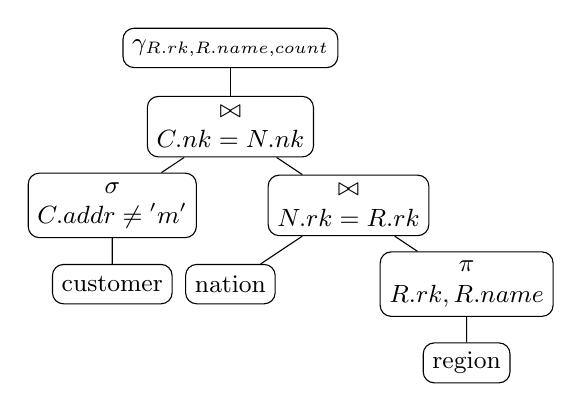
\begin{tikzpicture}[
  level distance=1cm,
  sibling distance=3cm,
  every node/.style={
    draw,
    rounded corners,
    align=center,
    minimum height=0.5cm,
    font=\small
  }
]
\node{$\gamma_{R.rk, R.name, count}$}
  child {
    node{$\bowtie$\\$C.nk = N.nk$}
    child {
      node{$\sigma$\\$C.addr \neq \text{'m'}$}
      child {
        node{customer}
      }
    }
    child {
      node{$\bowtie$\\$N.rk = R.rk$}
      child {
        node{nation}
      }
      child {
        node{$\pi$\\$R.rk, R.name$}
        child {
          node{region}
        }
      }
    }
  };
\end{tikzpicture}

\spacing
\noindent
We start with a left entity $E = customer$. We build this query up until we hit the merge operation, where we then start bottom-up from $nation$, stepping once again recursively building up the $region$ query. We join each atomic query (a specific set of sub-trees) together with merge operations, appending a groupby operation to the outer-most query.

\spacing
\noindent
Queries are \textit{always} built bottom-up starting from individual entities (or tables) described by the schema $S$. Each query has a sole acting entity, and we combine these atomic queries with merge operations to form one large and complex query, which may act on all entities described by $S$.

\spacing
\noindent
We're able sustain such complex recursion trees that maintain query validity simply because we preserve join columns all the way down. The projection generation process always takes into account $R$, a required column set.

\subsubsection*{Groupby $(\gamma)$}

For simplicity, we \textit{always} generate the group-by with an aggregation. Since this is always appended at the end of the outer-most query, we need not worry about required columns, so we pick a random subset from our available columns with a mapping of columns to aggregation functions.

\spacing
\begin{lstlisting}
set X to rand(1, min($C_{\gamma}$, |$C$|))

select a subset $G_{S} \subseteq C$, |$G_{S}$| = X

set $A$ to be C - $G_{S}$

if A is empty
  group by on $G_S$, without aggregation

set Y to be rand(1, min($C_{\Sigma}$, |A|))

select a subset $A_{S} \subseteq A$, |$A_{S}|$ = Y

set $F$ to be an empty mapping

for each column $\in$ $A_{S}$
  map column -> a function, in $F$

group by on $G_S$, aggregate with $F$
\end{lstlisting}

\spacing
\noindent
The mapping of columns to a function should be done knowing the columns type. For instance, a column whose type is string should not get mapped with $mean$. This mapping can be defined statically in code, associating column types with appropriate functions.

\subsection*{Output}

The algorithm outputs a set of operations, call it the resulting operation set $O_{R}$ \text{where} $\forall o \in O_{R}, o \in O$.

\section{Software Implementation}

We provide a full and comprehensive Python command-line tool and library that implements the aforementioned algorithm, called \textbf{pqg}, that lets users generate thousands of complex queries for their schemas very quickly.

\subsection*{Results}

\subsection*{Benchmarks}

\section{Conclusion}

\section{References}

\end{document}
